\documentclass[11pt,a4paper]{article}

% Packages
\usepackage{amsmath}
\usepackage{amssymb}
\usepackage{amsthm}
\usepackage[margin=1in]{geometry}
\usepackage{enumitem}
\usepackage{tikz}
\usepackage{pgfplots}
\usepackage{xcolor}
\pgfplotsset{compat=1.18}

% Custom commands
\newcommand{\stage}[1]{\textbf{\textcolor{blue}{#1}}}

% Title information
\title{Exercise Sheet 3: Bifurcations\\
Question 8 - Complete Solution}
\author{Methods of Applied Mathematics}
\date{}

\begin{document}

\maketitle

\section*{Problem Statement}

Determine what bifurcation happens as $\mu$ changes in the system:
\[
\frac{dx}{dt} = x - x^3 + \mu
\]

\vspace{10pt}
\hrule
\vspace{10pt}

\section{Step 1: Analyze System Structure}

\subsection*{Rewrite equilibrium condition}

For equilibria, set $\dot{x} = 0$:
\[
x - x^3 + \mu = 0
\]

Rearranging:
\[
x^3 - x = \mu
\]

or equivalently:
\[
x^3 = x + \mu
\]

\subsection*{Geometric interpretation}

Define $h(x) = x^3 - x$. Then equilibria occur where:
\[
h(x) = \mu
\]

This means equilibria are intersections of the cubic curve $y = x^3 - x$ with horizontal line $y = \mu$.

\subsection*{XYZ Analysis of Problem Structure}

\begin{itemize}[leftmargin=*]
\item \stage{STAGE X (What we have):} A 1D system where equilibria are roots of cubic equation. The parameter $\mu$ appears additively, shifting the equilibrium equation vertically.

\item \stage{STAGE Y (Why this approach):} Unlike previous problems where equilibria had explicit formulas, this cubic generally requires graphical/numerical analysis. The key insight: view the problem as finding where a fixed cubic curve $h(x) = x^3 - x$ intersects a moving horizontal line $y = \mu$. As $\mu$ varies:
\begin{itemize}
\item High horizontal line ($\mu$ large): may intersect cubic once
\item Medium height: may intersect three times
\item Low horizontal line ($\mu$ very negative): may intersect once
\end{itemize}
The number of intersections (equilibria) changes when the line becomes tangent to the cubic - this signals a fold bifurcation where two equilibria collide and annihilate.

\item \stage{STAGE Z (What to find):} We need to:
\begin{enumerate}
\item Find critical points of $h(x)$ (local max/min)
\item Evaluate $h$ at these critical points to find bifurcation values of $\mu$
\item Determine stability of equilibria in each parameter regime
\item Identify the bifurcation type(s)
\end{enumerate}
\end{itemize}

\vspace{10pt}
\hrule
\vspace{10pt}

\section{Step 2: Analyze the Cubic Function}

\subsection*{Define the function}

\[
h(x) = x^3 - x
\]

\subsection*{Factor the function}

\[
h(x) = x(x^2 - 1) = x(x-1)(x+1)
\]

Roots of $h$: $x = -1, 0, 1$

\subsection*{Find critical points}

\[
h'(x) = 3x^2 - 1
\]

Set $h'(x) = 0$:
\[
3x^2 = 1 \quad \Rightarrow \quad x^2 = \frac{1}{3} \quad \Rightarrow \quad x = \pm\frac{1}{\sqrt{3}}
\]

\subsection*{Classify critical points}

Second derivative:
\[
h''(x) = 6x
\]

At $x = 1/\sqrt{3}$: $h''(1/\sqrt{3}) = 6/\sqrt{3} = 2\sqrt{3} > 0$ → Local minimum

At $x = -1/\sqrt{3}$: $h''(-1/\sqrt{3}) = -6/\sqrt{3} = -2\sqrt{3} < 0$ → Local maximum

\subsection*{Evaluate $h$ at critical points}

\textbf{At local minimum $x = 1/\sqrt{3}$:}
\begin{align*}
h\left(\frac{1}{\sqrt{3}}\right) &= \left(\frac{1}{\sqrt{3}}\right)^3 - \frac{1}{\sqrt{3}} \\
&= \frac{1}{3\sqrt{3}} - \frac{1}{\sqrt{3}} \\
&= \frac{1}{3\sqrt{3}} - \frac{3}{3\sqrt{3}} \\
&= -\frac{2}{3\sqrt{3}} = -\frac{2\sqrt{3}}{9}
\end{align*}

\textbf{At local maximum $x = -1/\sqrt{3}$:}
\begin{align*}
h\left(-\frac{1}{\sqrt{3}}\right) &= -\left(\frac{1}{\sqrt{3}}\right)^3 + \frac{1}{\sqrt{3}} \\
&= -\frac{1}{3\sqrt{3}} + \frac{1}{\sqrt{3}} \\
&= -\frac{1}{3\sqrt{3}} + \frac{3}{3\sqrt{3}} \\
&= \frac{2}{3\sqrt{3}} = \frac{2\sqrt{3}}{9}
\end{align*}

\subsection*{Summary of cubic properties}

\[
\boxed{
\begin{array}{rcl}
\text{Local maximum:} & x = -\dfrac{1}{\sqrt{3}}, & h = \dfrac{2\sqrt{3}}{9} \approx 0.3849 \\[10pt]
\text{Local minimum:} & x = \dfrac{1}{\sqrt{3}}, & h = -\dfrac{2\sqrt{3}}{9} \approx -0.3849
\end{array}
}
\]

\subsection*{XYZ Analysis of Cubic Structure}

\begin{itemize}[leftmargin=*]
\item \stage{STAGE X (What we found):} The cubic $h(x) = x^3 - x$ has two critical points: a local max at $x = -1/\sqrt{3}$ with value $2\sqrt{3}/9$, and a local min at $x = 1/\sqrt{3}$ with value $-2\sqrt{3}/9$.

\item \stage{STAGE Y (Why these values matter):} These critical values of $h$ are where horizontal lines become tangent to the cubic curve. They represent threshold values of $\mu$:
\begin{itemize}
\item If $\mu > 2\sqrt{3}/9$: line $y = \mu$ is above the local max, intersecting cubic only once (far right)
\item If $\mu = 2\sqrt{3}/9$: line is tangent at local max (two equilibria touch)
\item If $-2\sqrt{3}/9 < \mu < 2\sqrt{3}/9$: line intersects cubic three times
\item If $\mu = -2\sqrt{3}/9$: line is tangent at local min (two equilibria touch)
\item If $\mu < -2\sqrt{3}/9$: line is below local min, intersecting cubic only once (far left)
\end{itemize}
The tangency points are fold bifurcations where pairs of equilibria collide and annihilate.

\item \stage{STAGE Z (What this means):} The system undergoes TWO fold bifurcations as $\mu$ varies. Between them, three equilibria coexist; outside, only one equilibrium exists. This is richer structure than a single fold bifurcation.
\end{itemize}

\vspace{10pt}
\hrule
\vspace{10pt}

\section{Step 3: Count Equilibria by Parameter Range}

\subsection*{Number of real roots}

The equation $x^3 - x = \mu$ has:

\begin{align*}
\mu > \frac{2\sqrt{3}}{9}: \quad & \boxed{\text{1 equilibrium}} \\[5pt]
\mu = \frac{2\sqrt{3}}{9}: \quad & \boxed{\text{2 equilibria (one repeated)}} \\[5pt]
-\frac{2\sqrt{3}}{9} < \mu < \frac{2\sqrt{3}}{9}: \quad & \boxed{\text{3 equilibria}} \\[5pt]
\mu = -\frac{2\sqrt{3}}{9}: \quad & \boxed{\text{2 equilibria (one repeated)}} \\[5pt]
\mu < -\frac{2\sqrt{3}}{9}: \quad & \boxed{\text{1 equilibrium}}
\end{align*}

\subsection*{Sketch of cubic and horizontal lines}

\begin{center}
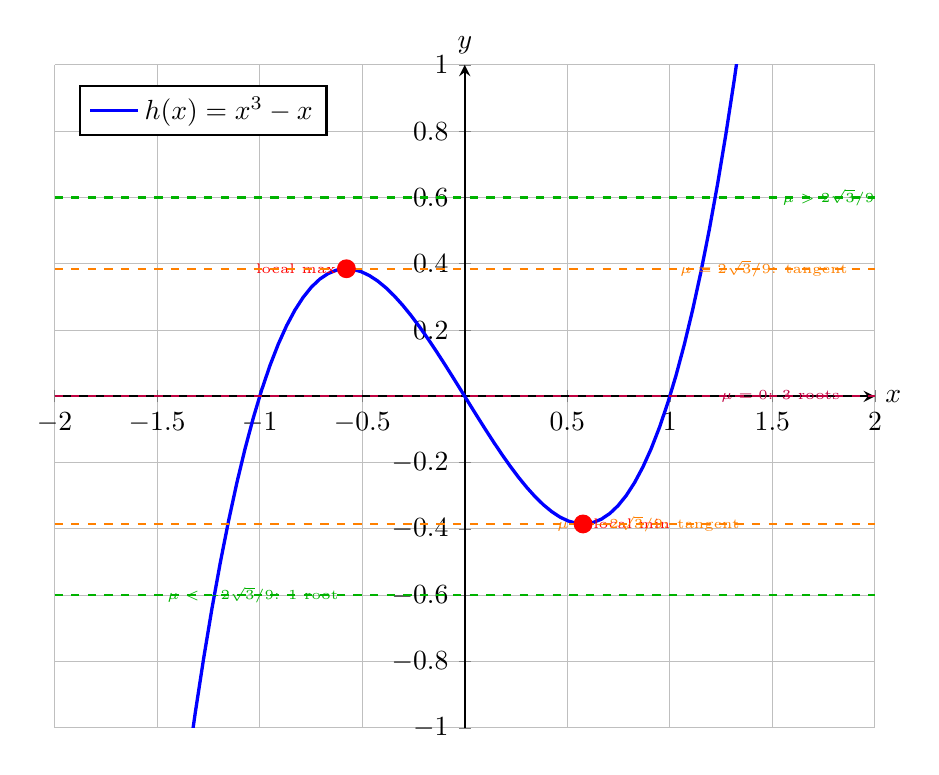
\begin{tikzpicture}
\begin{axis}[
    width=12cm,
    height=10cm,
    xlabel={$x$},
    ylabel={$y$},
    xmin=-2, xmax=2,
    ymin=-1, ymax=1,
    grid=major,
    axis lines=middle,
    thick,
    every axis x label/.style={at={(current axis.right of origin)},anchor=west},
    every axis y label/.style={at={(current axis.above origin)},anchor=south},
    legend pos=north west
]

% Cubic curve h(x) = x^3 - x
\addplot[blue, very thick, domain=-2:2, samples=100] {x^3 - x};
\addlegendentry{$h(x) = x^3 - x$}

% Critical points
\addplot[mark=*, mark size=3pt, red, only marks] coordinates {(-0.577, 0.385)};
\addplot[mark=*, mark size=3pt, red, only marks] coordinates {(0.577, -0.385)};
\node[red, font=\tiny, anchor=east] at (axis cs:-0.577,0.385) {local max};
\node[red, font=\tiny, anchor=west] at (axis cs:0.577,-0.385) {local min};

% Horizontal lines for different mu
\addplot[green!70!black, dashed, domain=-2:2] {0.6};
\node[green!70!black, font=\tiny, anchor=west] at (axis cs:1.5,0.6) {$\mu > 2\sqrt{3}/9$: 1 root};

\addplot[orange, dashed, domain=-2:2] {0.385};
\node[orange, font=\tiny, anchor=west] at (axis cs:1,0.385) {$\mu = 2\sqrt{3}/9$: tangent};

\addplot[purple, dashed, domain=-2:2] {0};
\node[purple, font=\tiny, anchor=west] at (axis cs:1.2,0) {$\mu = 0$: 3 roots};

\addplot[orange, dashed, domain=-2:2] {-0.385};
\node[orange, font=\tiny, anchor=west] at (axis cs:0.4,-0.385) {$\mu = -2\sqrt{3}/9$: tangent};

\addplot[green!70!black, dashed, domain=-2:2] {-0.6};
\node[green!70!black, font=\tiny, anchor=west] at (axis cs:-1.5,-0.6) {$\mu < -2\sqrt{3}/9$: 1 root};

\end{axis}
\end{tikzpicture}
\end{center}

\subsection*{XYZ Analysis of Equilibrium Count}

\begin{itemize}[leftmargin=*]
\item \stage{STAGE X (What the diagram shows):} The cubic curve and various horizontal lines. Lines above the local max or below the local min intersect once; lines between the extrema intersect three times.

\item \stage{STAGE Y (Why count changes):} The fundamental theorem of algebra guarantees a cubic has three roots (counting multiplicities, including complex). For our equation $x^3 - x - \mu = 0$:
\begin{itemize}
\item When $\mu$ is extreme: one real root, two complex conjugate roots
\item When $\mu$ is intermediate: three distinct real roots
\item At transition ($\mu = \pm 2\sqrt{3}/9$): three real roots, but two coincide (repeated root)
\end{itemize}
The complex roots become real as $\mu$ enters the interval $(-2\sqrt{3}/9, 2\sqrt{3}/9)$, and the transition happens via fold bifurcation where a pair of real roots emerges from (or disappears into) the complex plane.

\item \stage{STAGE Z (What this predicts):} Two fold bifurcations occur:
\begin{enumerate}
\item At $\mu = 2\sqrt{3}/9$: fold at $x = -1/\sqrt{3}$ (left side of curve)
\item At $\mu = -2\sqrt{3}/9$: fold at $x = 1/\sqrt{3}$ (right side of curve)
\end{enumerate}
Between bifurcations, the system has three equilibria. We now need to determine their stabilities.
\end{itemize}

\vspace{10pt}
\hrule
\vspace{10pt}

\section{Step 4: Determine Stability}

\subsection*{Compute derivative}

For $f(x) = x - x^3 + \mu$:
\[
f'(x) = 1 - 3x^2
\]

\subsection*{Stability criterion}

\begin{itemize}
\item $f'(x) < 0$: stable (flow toward equilibrium)
\item $f'(x) > 0$: unstable (flow away from equilibrium)
\item $f'(x) = 0$: neutral (bifurcation point)
\end{itemize}

\subsection*{Analyze sign of $f'(x)$}

\[
f'(x) = 1 - 3x^2 < 0 \quad \Leftrightarrow \quad x^2 > \frac{1}{3} \quad \Leftrightarrow \quad |x| > \frac{1}{\sqrt{3}}
\]

So:
\begin{align*}
|x| > \frac{1}{\sqrt{3}}: \quad & f'(x) < 0 \quad \Rightarrow \quad \text{STABLE} \\
|x| < \frac{1}{\sqrt{3}}: \quad & f'(x) > 0 \quad \Rightarrow \quad \text{UNSTABLE} \\
|x| = \frac{1}{\sqrt{3}}: \quad & f'(x) = 0 \quad \Rightarrow \quad \text{NEUTRAL (bifurcation)}
\end{align*}

\subsection*{Stability pattern for three equilibria}

When three equilibria exist (for $-2\sqrt{3}/9 < \mu < 2\sqrt{3}/9$), denote them as $x_L < x_M < x_R$ (left, middle, right):

\begin{itemize}
\item $x_L$ is far left: $x_L < -1/\sqrt{3}$, so $|x_L| > 1/\sqrt{3}$ → \textbf{Stable}
\item $x_M$ is in middle: $|x_M| < 1/\sqrt{3}$ → \textbf{Unstable}
\item $x_R$ is far right: $x_R > 1/\sqrt{3}$, so $|x_R| > 1/\sqrt{3}$ → \textbf{Stable}
\end{itemize}

\subsection*{Stability at bifurcation points}

\textbf{At $\mu = 2\sqrt{3}/9$:} Two equilibria at/near $x = -1/\sqrt{3}$
\begin{itemize}
\item One at $x = -1/\sqrt{3}$ exactly: $f'(-1/\sqrt{3}) = 0$ (neutral)
\item One slightly left: $f' < 0$ (stable)
\end{itemize}

\textbf{At $\mu = -2\sqrt{3}/9$:} Two equilibria at/near $x = 1/\sqrt{3}$
\begin{itemize}
\item One at $x = 1/\sqrt{3}$ exactly: $f'(1/\sqrt{3}) = 0$ (neutral)
\item One slightly right: $f' < 0$ (stable)
\end{itemize}

\subsection*{XYZ Analysis of Stability}

\begin{itemize}[leftmargin=*]
\item \stage{STAGE X (What we found):} The stability depends only on position: equilibria with $|x| > 1/\sqrt{3}$ are stable, those with $|x| < 1/\sqrt{3}$ are unstable. When three equilibria exist, the pattern is stable-unstable-stable.

\item \stage{STAGE Y (Why this pattern):} The derivative $f'(x) = 1 - 3x^2$ is a downward-opening parabola in $x$:
\begin{itemize}
\item Positive near $x = 0$ (unstable equilibria)
\item Negative for $|x|$ large (stable equilibria)
\item Zero at $x = \pm 1/\sqrt{3}$ (bifurcation points)
\end{itemize}
The physical interpretation: for $|x|$ small, the linear term $x$ dominates (positive coefficient → unstable). For $|x|$ large, the cubic term $-x^3$ dominates (negative coefficient for large $|x|$ → stable). The balance point is at $|x| = 1/\sqrt{3}$.

This means equilibria born in fold bifurcations inherit predictable stabilities based on their positions. At the right fold ($x = 1/\sqrt{3}$), a stable equilibrium (with $x > 1/\sqrt{3}$) collides with an unstable one (with $x < 1/\sqrt{3}$). Similarly at the left fold.

\item \stage{STAGE Z (What this means for dynamics):} In the three-equilibria regime, the middle equilibrium is a separatrix:
\begin{itemize}
\item Initial conditions $x < x_M$: flow toward $x_L$ (left stable equilibrium)
\item Initial conditions $x > x_M$: flow toward $x_R$ (right stable equilibrium)
\end{itemize}
The unstable middle equilibrium divides the phase space into two basins of attraction. At fold bifurcations, these basins merge or separate as equilibria are created/destroyed.
\end{itemize}

\vspace{10pt}
\hrule
\vspace{10pt}

\section{Step 5: Verify Fold Bifurcation Conditions}

\subsection*{Left fold at $\mu = 2\sqrt{3}/9$, $x = -1/\sqrt{3}$}

For $f(x, \mu) = x - x^3 + \mu$:

\textbf{(B1) Equilibrium exists:}
\[
f\left(-\frac{1}{\sqrt{3}}, \frac{2\sqrt{3}}{9}\right) = -\frac{1}{\sqrt{3}} - \left(-\frac{1}{\sqrt{3}}\right)^3 + \frac{2\sqrt{3}}{9} = -\frac{1}{\sqrt{3}} + \frac{1}{3\sqrt{3}} + \frac{2\sqrt{3}}{9}
\]
\[
= -\frac{3}{3\sqrt{3}} + \frac{1}{3\sqrt{3}} + \frac{2\sqrt{3}}{9} = -\frac{2}{3\sqrt{3}} + \frac{2\sqrt{3}}{9} = -\frac{2\sqrt{3}}{9} + \frac{2\sqrt{3}}{9} = 0 \quad \checkmark
\]

\textbf{(B2) Zero eigenvalue:}
\[
\frac{\partial f}{\partial x}\bigg|_{x=-1/\sqrt{3}} = 1 - 3\left(\frac{1}{3}\right) = 1 - 1 = 0 \quad \checkmark
\]

\textbf{(G1) Second derivative nonzero:}
\[
\frac{\partial^2 f}{\partial x^2} = -6x \quad \Rightarrow \quad \frac{\partial^2 f}{\partial x^2}\bigg|_{x=-1/\sqrt{3}} = -6 \cdot \left(-\frac{1}{\sqrt{3}}\right) = \frac{6}{\sqrt{3}} = 2\sqrt{3} \neq 0 \quad \checkmark
\]

\textbf{(G2) Parameter derivative nonzero:}
\[
\frac{\partial f}{\partial \mu} = 1 \quad \Rightarrow \quad \frac{\partial f}{\partial \mu}\bigg|_{\text{any point}} = 1 \neq 0 \quad \checkmark
\]

\subsection*{Right fold at $\mu = -2\sqrt{3}/9$, $x = 1/\sqrt{3}$}

For $f(x, \mu) = x - x^3 + \mu$:

\textbf{(B1) Equilibrium exists:}
\[
f\left(\frac{1}{\sqrt{3}}, -\frac{2\sqrt{3}}{9}\right) = \frac{1}{\sqrt{3}} - \left(\frac{1}{\sqrt{3}}\right)^3 - \frac{2\sqrt{3}}{9} = \frac{1}{\sqrt{3}} - \frac{1}{3\sqrt{3}} - \frac{2\sqrt{3}}{9}
\]
\[
= \frac{3}{3\sqrt{3}} - \frac{1}{3\sqrt{3}} - \frac{2\sqrt{3}}{9} = \frac{2}{3\sqrt{3}} - \frac{2\sqrt{3}}{9} = \frac{2\sqrt{3}}{9} - \frac{2\sqrt{3}}{9} = 0 \quad \checkmark
\]

\textbf{(B2) Zero eigenvalue:}
\[
\frac{\partial f}{\partial x}\bigg|_{x=1/\sqrt{3}} = 1 - 3\left(\frac{1}{3}\right) = 0 \quad \checkmark
\]

\textbf{(G1) Second derivative nonzero:}
\[
\frac{\partial^2 f}{\partial x^2}\bigg|_{x=1/\sqrt{3}} = -6 \cdot \frac{1}{\sqrt{3}} = -\frac{6}{\sqrt{3}} = -2\sqrt{3} \neq 0 \quad \checkmark
\]

\textbf{(G2) Parameter derivative nonzero:}
\[
\frac{\partial f}{\partial \mu} = 1 \neq 0 \quad \checkmark
\]

\subsection*{Conclusion}

\[
\boxed{
\begin{array}{l}
\text{FOLD BIFURCATION at } \mu = \dfrac{2\sqrt{3}}{9}, \, x = -\dfrac{1}{\sqrt{3}} \\[10pt]
\text{FOLD BIFURCATION at } \mu = -\dfrac{2\sqrt{3}}{9}, \, x = \dfrac{1}{\sqrt{3}}
\end{array}
}
\]

\subsection*{XYZ Analysis of Verification}

\begin{itemize}[leftmargin=*]
\item \stage{STAGE X (What we verified):} Both bifurcation points satisfy all four conditions (B1, B2, G1, G2) for fold bifurcations.

\item \stage{STAGE Y (Why two folds):} The cubic equation can have up to two pairs of equilibria that collide. Each collision is independent:
\begin{itemize}
\item Left fold: Occurs at local maximum of $h(x)$. As $\mu$ decreases through $2\sqrt{3}/9$, two equilibria emerge on the left branch
\item Right fold: Occurs at local minimum of $h(x)$. As $\mu$ increases through $-2\sqrt{3}/9$, two equilibria emerge on the right branch
\end{itemize}
The sign difference in $\partial^2 f/\partial x^2$ ($+2\sqrt{3}$ vs $-2\sqrt{3}$) reflects the different curvatures at left (max) and right (min) critical points. But both are fold bifurcations - the sign of second derivative just indicates which branch is stable.

\item \stage{STAGE Z (What this represents):} Systems with multiple fold bifurcations exhibit hysteresis and bistability:
\begin{itemize}
\item For intermediate $\mu$: two stable states coexist with one unstable separatrix
\item Slowly increasing $\mu$ from $\mu \ll 0$: system stays on right stable branch until right fold at $\mu = -2\sqrt{3}/9$, then jumps to left stable branch
\item Slowly decreasing $\mu$ from $\mu \gg 0$: system stays on left stable branch until left fold at $\mu = 2\sqrt{3}/9$, then jumps to right stable branch
\end{itemize}
The path taken depends on history - this is hysteresis, common in mechanical buckling, optical bistability, and ecological regime shifts.
\end{itemize}

\vspace{10pt}
\hrule
\vspace{10pt}

\section{Step 6: Bifurcation Diagram}

\subsection*{Equilibrium curves}

From $x^3 - x = \mu$, we can plot $x$ vs $\mu$.

Alternatively, parametrize by $x$ and compute $\mu(x) = x^3 - x$:

\begin{itemize}
\item For $x < -1/\sqrt{3}$: upper-left branch (stable)
\item At $x = -1/\sqrt{3}$: fold point, $\mu = 2\sqrt{3}/9$
\item For $-1/\sqrt{3} < x < 1/\sqrt{3}$: middle branch (unstable)
\item At $x = 1/\sqrt{3}$: fold point, $\mu = -2\sqrt{3}/9$
\item For $x > 1/\sqrt{3}$: lower-right branch (stable)
\end{itemize}

\subsection*{Bifurcation diagram: $\mu$ vs $x$}

\begin{center}
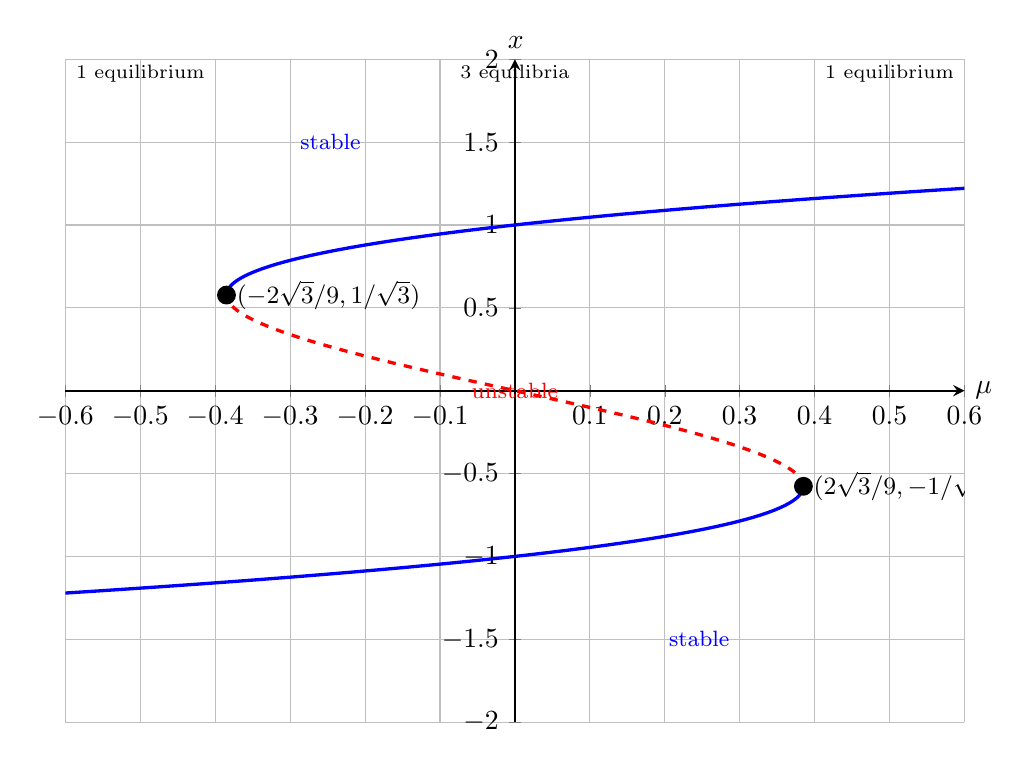
\begin{tikzpicture}
\begin{axis}[
    width=13cm,
    height=10cm,
    xlabel={$\mu$},
    ylabel={$x$},
    xmin=-0.6, xmax=0.6,
    ymin=-2, ymax=2,
    grid=major,
    axis lines=middle,
    thick,
    every axis x label/.style={at={(current axis.right of origin)},anchor=west},
    every axis y label/.style={at={(current axis.above origin)},anchor=south}
]

% Parametric curve: mu = x^3 - x
% Left stable branch
\addplot[blue, very thick, solid, domain=-2:-0.577, samples=100] ({x^3 - x}, {x});

% Middle unstable branch
\addplot[red, very thick, dashed, domain=-0.577:0.577, samples=100] ({x^3 - x}, {x});

% Right stable branch
\addplot[blue, very thick, solid, domain=0.577:2, samples=100] ({x^3 - x}, {x});

% Fold bifurcation points
\addplot[mark=*, mark size=3pt, black, only marks] coordinates {(0.385, -0.577)};
\node[font=\small, anchor=west] at (axis cs:0.385,-0.577) {$(2\sqrt{3}/9, -1/\sqrt{3})$};

\addplot[mark=*, mark size=3pt, black, only marks] coordinates {(-0.385, 0.577)};
\node[font=\small, anchor=west] at (axis cs:-0.385,0.577) {$(-2\sqrt{3}/9, 1/\sqrt{3})$};

% Labels
\node[blue, font=\footnotesize, anchor=east] at (axis cs:0.3,-1.5) {stable};
\node[red, font=\footnotesize] at (axis cs:0,0) {unstable};
\node[blue, font=\footnotesize, anchor=west] at (axis cs:-0.3,1.5) {stable};

% Region labels
\node[font=\scriptsize, anchor=south] at (axis cs:-0.5,1.8) {1 equilibrium};
\node[font=\scriptsize, anchor=south] at (axis cs:0,1.8) {3 equilibria};
\node[font=\scriptsize, anchor=south] at (axis cs:0.5,1.8) {1 equilibrium};

\end{axis}
\end{tikzpicture}
\end{center}

\subsection*{XYZ Analysis of Bifurcation Diagram}

\begin{itemize}[leftmargin=*]
\item \stage{STAGE X (What the diagram shows):} An "S-shaped" or "N-shaped" curve (depending on orientation). Two fold points where the curve turns back on itself. Solid lines (stable) on outer branches, dashed line (unstable) on middle branch.

\item \stage{STAGE Y (Why this shape):} The curve is simply the graph of $\mu = x^3 - x$ rotated 90° (plotted with axes swapped). The S-shape comes from the cubic function:
\begin{itemize}
\item For $\mu$ far left: line $y = \mu$ intersects cubic once (upper left) → single equilibrium at large negative $x$
\item As $\mu$ increases to $-2\sqrt{3}/9$: line rises to tangency point → fold bifurcation, two new equilibria born
\item For intermediate $\mu$: line intersects cubic three times → three coexisting equilibria
\item As $\mu$ increases to $2\sqrt{3}/9$: line reaches upper tangency → second fold bifurcation, two equilibria annihilate
\item For $\mu$ far right: line intersects once (lower right) → single equilibrium at large positive $x$
\end{itemize}
The middle branch "folds back" because $\mu(x) = x^3 - x$ is not monotonic - it decreases then increases.

\item \stage{STAGE Z (What this means for control):} Reading vertically at fixed $\mu$:
\begin{itemize}
\item Outside folds: one equilibrium (unique stable state)
\item Between folds: three equilibria (bistability - two stable attractors separated by unstable saddle)
\end{itemize}
Reading horizontally shows hysteresis: slowly varying $\mu$ causes system to jump discontinuously at fold points. The system "remembers" which branch it's on. Applications include:
\begin{itemize}
\item Mechanical systems: beam buckling under load
\item Optical systems: bistable lasers
\item Climate models: ice-albedo feedback leading to abrupt transitions
\item Ecological systems: lake eutrophication with multiple stable states
\end{itemize}
\end{itemize}

\vspace{10pt}
\hrule
\vspace{10pt}

\section{Step 7: Phase Portraits}

\subsection*{Five representative scenarios}

\begin{center}
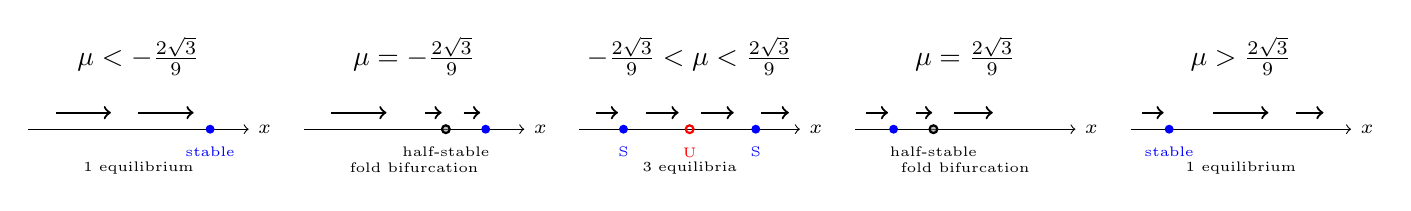
\begin{tikzpicture}[scale=0.7]
% mu << -2sqrt(3)/9
\begin{scope}[shift={(0,0)}]
\draw[->] (-2,0) -- (2,0) node[right, font=\scriptsize] {$x$};
\node[above] at (0,0.8) {$\mu < -\frac{2\sqrt{3}}{9}$};
% One stable equilibrium far right
\filldraw[blue] (1.3,0) circle (2pt) node[below=3pt, font=\tiny] {stable};
\draw[->, thick] (-1.5,0.3) -- (-0.5,0.3);
\draw[->, thick] (0,0.3) -- (1,0.3);
\node[font=\tiny] at (0,-0.7) {1 equilibrium};
\end{scope}

% mu = -2sqrt(3)/9
\begin{scope}[shift={(5,0)}]
\draw[->] (-2,0) -- (2,0) node[right, font=\scriptsize] {$x$};
\node[above] at (0,0.8) {$\mu = -\frac{2\sqrt{3}}{9}$};
% Half-stable at fold point
\draw[thick, fill=gray, fill opacity=0.5] (0.577,0) circle (2pt);
\node[below=3pt, font=\tiny] at (0.577,0) {half-stable};
\filldraw[blue] (1.3,0) circle (2pt);
\draw[->, thick] (-1.5,0.3) -- (-0.5,0.3);
\draw[->, thick] (0.2,0.3) -- (0.5,0.3);
\draw[->, thick] (0.9,0.3) -- (1.2,0.3);
\node[font=\tiny] at (0,-0.7) {fold bifurcation};
\end{scope}

% Intermediate
\begin{scope}[shift={(10,0)}]
\draw[->] (-2,0) -- (2,0) node[right, font=\scriptsize] {$x$};
\node[above] at (0,0.8) {$-\frac{2\sqrt{3}}{9} < \mu < \frac{2\sqrt{3}}{9}$};
% Three equilibria: S-U-S
\filldraw[blue] (-1.2,0) circle (2pt) node[below=3pt, font=\tiny] {S};
\draw[red, thick] (0,0) circle (2pt) node[below=3pt, font=\tiny] {U};
\filldraw[blue] (1.2,0) circle (2pt) node[below=3pt, font=\tiny] {S};
\draw[->, thick] (-1.7,0.3) -- (-1.3,0.3);
\draw[->, thick] (-0.8,0.3) -- (-0.2,0.3);
\draw[->, thick] (0.2,0.3) -- (0.8,0.3);
\draw[->, thick] (1.3,0.3) -- (1.8,0.3);
\node[font=\tiny] at (0,-0.7) {3 equilibria};
\end{scope}

% mu = 2sqrt(3)/9
\begin{scope}[shift={(15,0)}]
\draw[->] (-2,0) -- (2,0) node[right, font=\scriptsize] {$x$};
\node[above] at (0,0.8) {$\mu = \frac{2\sqrt{3}}{9}$};
% Half-stable at fold point
\filldraw[blue] (-1.3,0) circle (2pt);
\draw[thick, fill=gray, fill opacity=0.5] (-0.577,0) circle (2pt);
\node[below=3pt, font=\tiny] at (-0.577,0) {half-stable};
\draw[->, thick] (-1.8,0.3) -- (-1.4,0.3);
\draw[->, thick] (-0.9,0.3) -- (-0.6,0.3);
\draw[->, thick] (-0.2,0.3) -- (0.5,0.3);
\node[font=\tiny] at (0,-0.7) {fold bifurcation};
\end{scope}

% mu >> 2sqrt(3)/9
\begin{scope}[shift={(20,0)}]
\draw[->] (-2,0) -- (2,0) node[right, font=\scriptsize] {$x$};
\node[above] at (0,0.8) {$\mu > \frac{2\sqrt{3}}{9}$};
% One stable equilibrium far left
\filldraw[blue] (-1.3,0) circle (2pt) node[below=3pt, font=\tiny] {stable};
\draw[->, thick] (-1.8,0.3) -- (-1.4,0.3);
\draw[->, thick] (-0.5,0.3) -- (0.5,0.3);
\draw[->, thick] (1,0.3) -- (1.5,0.3);
\node[font=\tiny] at (0,-0.7) {1 equilibrium};
\end{scope}
\end{tikzpicture}
\end{center}

\subsection*{XYZ Analysis of Phase Portraits}

\begin{itemize}[leftmargin=*]
\item \stage{STAGE X (What we see):} The number and type of equilibria changing dramatically as $\mu$ varies. Single stable state → fold → three states (bistability) → fold → single stable state.

\item \stage{STAGE Y (Why these transitions):} The 1D flow $\dot{x} = x - x^3 + \mu$ has:
\begin{itemize}
\item \textbf{Far left regime}: $\mu$ very negative makes $\dot{x}$ negative for most $x$, except far right where $x$ term dominates → single stable equilibrium at large positive $x$
\item \textbf{Right fold ($\mu = -2\sqrt{3}/9$)}: Two equilibria merge at $x = 1/\sqrt{3}$. The derivative is zero there (half-stable point)
\item \textbf{Central regime}: Three equilibria coexist. The outer two are stable (large $|x|$ where $-x^3$ dominates), middle is unstable (small $|x|$ where $x$ dominates)
\item \textbf{Left fold ($\mu = 2\sqrt{3}/9$)}: Two equilibria merge at $x = -1/\sqrt{3}$
\item \textbf{Far right regime}: $\mu$ very positive makes $\dot{x}$ positive for most $x$, except far left where $-x^3$ term dominates → single stable equilibrium at large negative $x$
\end{itemize}

\item \stage{STAGE Z (What this means globally):} The system exhibits path dependence (hysteresis):
\begin{itemize}
\item Start with $\mu \ll 0$, system at stable equilibrium (far right)
\item Slowly increase $\mu$: system stays on right stable branch, passing through bistable region
\item At $\mu = 2\sqrt{3}/9$: right stable branch disappears in fold → system must jump to left stable branch
\item Continue increasing $\mu$: system remains on left stable branch
\item Now decrease $\mu$: system stays on left stable branch, retracing through bistable region
\item At $\mu = -2\sqrt{3}/9$: left stable branch disappears in fold → system must jump to right stable branch
\end{itemize}
The path followed going up differs from the path going down - this creates a hysteresis loop. The system "remembers" where it came from via which stable branch it occupies.
\end{itemize}

\vspace{10pt}
\hrule
\vspace{10pt}

\section{Summary}

\subsection*{System}

\[
\dot{x} = x - x^3 + \mu
\]

\subsection*{Bifurcations}

\[
\boxed{
\begin{array}{rcl}
\text{Fold at:} & \mu = \dfrac{2\sqrt{3}}{9} \approx 0.3849, & x = -\dfrac{1}{\sqrt{3}} \approx -0.5774 \\[10pt]
\text{Fold at:} & \mu = -\dfrac{2\sqrt{3}}{9} \approx -0.3849, & x = \dfrac{1}{\sqrt{3}} \approx 0.5774
\end{array}
}
\]

\subsection*{Equilibrium structure by parameter regime}

\begin{center}
\begin{tabular}{|c|c|c|}
\hline
\textbf{Parameter Range} & \textbf{Number} & \textbf{Stability Pattern} \\
\hline
$\mu < -2\sqrt{3}/9$ & 1 & Stable (far right) \\
\hline
$\mu = -2\sqrt{3}/9$ & 2 & Half-stable + stable \\
\hline
$-2\sqrt{3}/9 < \mu < 2\sqrt{3}/9$ & 3 & Stable–Unstable–Stable \\
\hline
$\mu = 2\sqrt{3}/9$ & 2 & Stable + half-stable \\
\hline
$\mu > 2\sqrt{3}/9$ & 1 & Stable (far left) \\
\hline
\end{tabular}
\end{center}

\subsection*{Key phenomena}

\begin{itemize}
\item \textbf{Bistability}: For $|\mu| < 2\sqrt{3}/9$, two stable attractors coexist
\item \textbf{Hysteresis}: System path depends on direction of parameter variation
\item \textbf{Catastrophic jumps}: At fold points, sudden transitions between distant stable states
\item \textbf{S-shaped bifurcation diagram}: Characteristic of systems with cubic nonlinearity
\end{itemize}

\subsection*{Physical interpretation}

This structure appears in:
\begin{itemize}
\item Buckled beams (displacement vs load)
\item Optical bistability (intensity vs detuning)
\item Climate tipping points (temperature vs forcing)
\item Ecological regime shifts (biomass vs nutrient input)
\end{itemize}

The two fold bifurcations create a parameter window of bistability between catastrophic transition thresholds.

\end{document}
